\appendix

\section*{Technical Appendices and Supplementary Material}

\noindent
- Section~\hyperref[app:benchmark]{A}: Benchmark and Evaluation Details \\
- Section~\hyperref[app:detail_results]{B}: Detailed Results \\
- Section~\hyperref[app:quantization-details]{C}: Quantization Details \\
- Section~\hyperref[app:analysis]{D}: Analysis: Why LLMs Cannot Reliably Generate High-Performance Kernels \\
- Section~\hyperref[app:artifacts]{E}: Artifacts: Transition Pairs for Repair and Optimization Analysis


\section{Benchmark and Evaluation Details}
\label{app:benchmark}

\subsection{Task List and Category Taxonomy}

\oursys contains 176 tasks spanning 15 fine-grained categories. Rather than organizing tasks by operator type, we group them by the \emph{type of knowledge required to produce a correct implementation}, enabling category-level analysis of systematic failure modes.

\paragraph{Direct specification tasks (Activation, Math).}
\textbf{Activation} (10) and \textbf{Math} (36) are primarily defined by explicit formulas or standard library semantics (e.g.\@, ReLU, softmax). Correctness largely reduces to faithful translation of the specification, with occasional subtleties in composition or numerical stability.

\paragraph{Parallel aggregation structures (Reduce, Pooling, Normalization).}
\textbf{Reduce} (6), \textbf{Pooling} (2), and \textbf{Normalization} (5) depend on aggregation over a defined scope (e.g., reduction axis or normalization domain). 
Errors typically arise from incorrect scope or inconsistent statistics; some variants extend to matrix-level aggregation (e.g., spectral normalization).

\paragraph{Structured multi-operand computation (MatrixMultiply, LinearAlgebra).}
\textbf{MatrixMultiply} (10) centers on structured two-operand computation, often combined with additional reductions. \textbf{LinearAlgebra} (17) involves decompositions (SVD, QR, LU) with coupled multi-output constraints (e.g., $A = U S V^H$), requiring consistency across outputs.

\paragraph{Indexed and spatial computation (Convolution, Index, SpatialOps).}
\textbf{Convolution} (2), \textbf{Index} (6), and \textbf{SpatialOps} (3) are dominated by address computation rather than value arithmetic. Convolution requires boundary-aware sliding windows; Index tasks involve gather/scatter or masked selection; SpatialOps rely on coordinate mapping and interpolation.

\paragraph{Compositional kernels (Fusion).}
\textbf{Fusion} (60) composes multiple operations within a single kernel. Correctness depends on preserving invariants across operation boundaries, especially when combining elementwise, reduction, and normalization steps.

\paragraph{Semantic contract categories (Loss, Optimizer, Random, Quantization).}
These categories require knowledge beyond direct formulas. \textbf{Loss} and \textbf{Optimizer} involve API-level contracts (e.g., reduction modes, state updates). \textbf{Random} includes both stochastic sampling and deterministic tensor factories (e.g., \texttt{logspace}), requiring consistency under seeding and device semantics. \textbf{Quantization} follows an approximation contract, evaluated by multiple precision metrics rather than exact equality.

\paragraph{Discussion.}
These categories reflect different types of knowledge: explicit specifications, structured parallel patterns, compositional reasoning, and contract-level semantics. 
We hypothesize that the latter are less consistently represented in pretraining data, which may explain their lower correctness in Section~\ref{sec:category_correctness}.

\begin{figure*}[t]
    \centering
    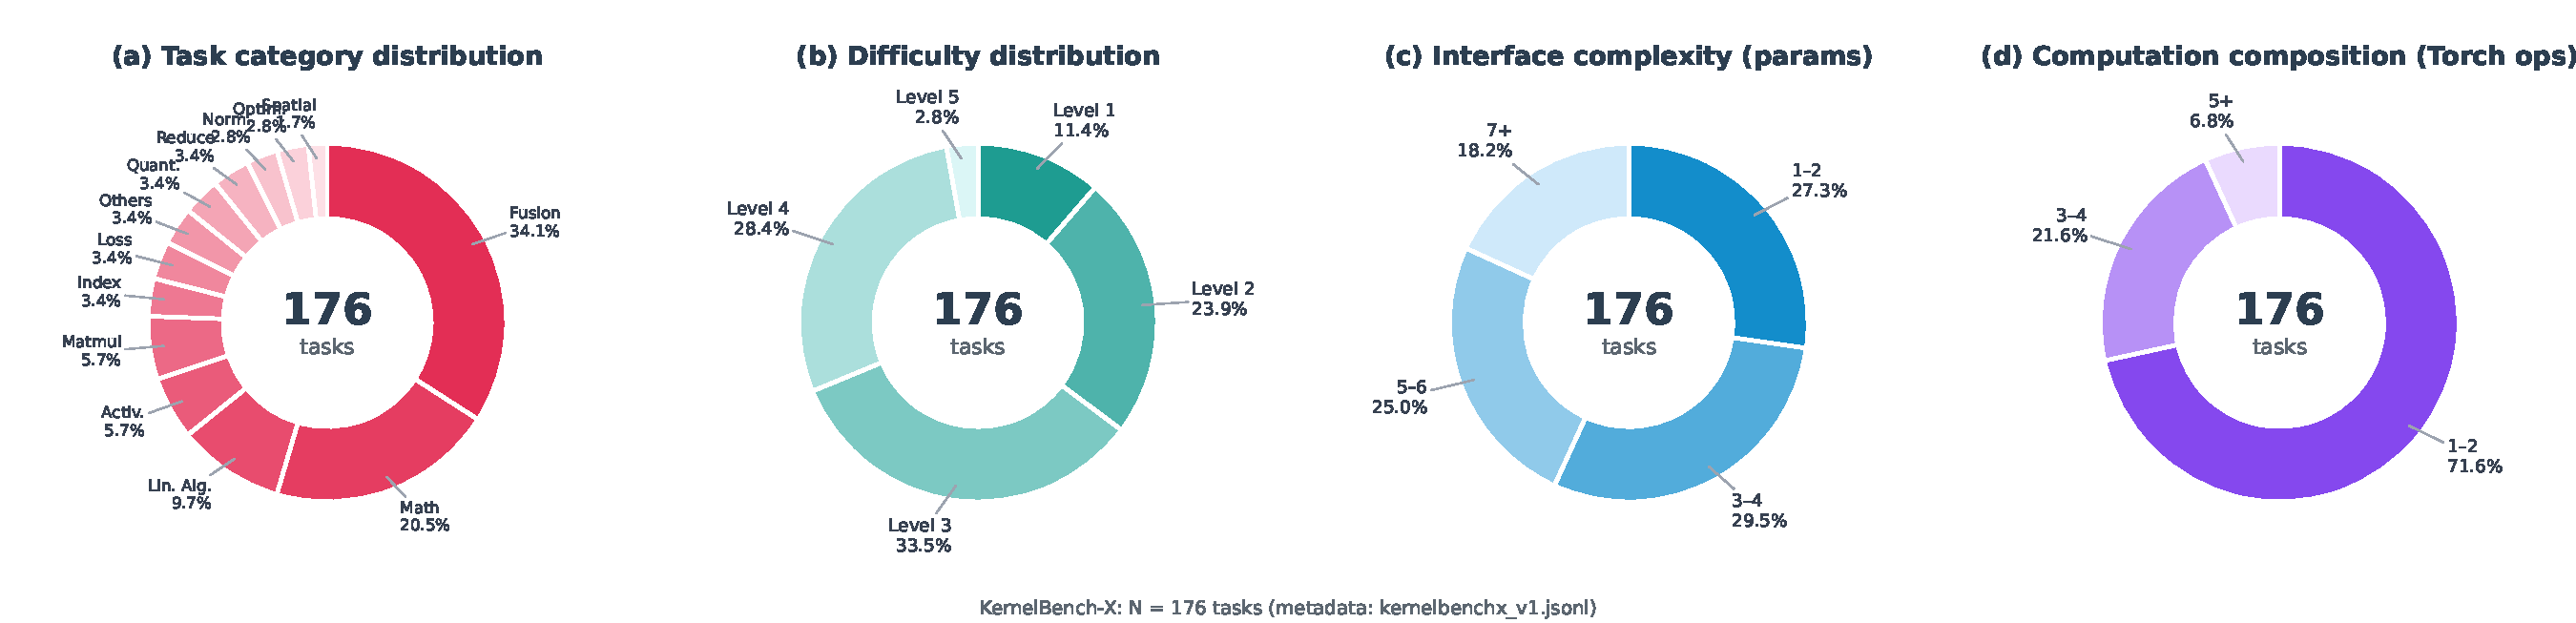
\includegraphics[width=0.95\textwidth]{src/figs/benchmark_overview.pdf}
    \caption{Overview of \oursys benchmark structure.}
    \label{fig:benchmark_overview}
\end{figure*}


\subsection{Call Accuracy}

A task is counted as passing the call stage only if the generated prediction is non-empty, exports a valid kernel entry according to the benchmark’s AST-based kernel-entry check, and executes successfully under the call harness. For Quantization tasks, an additional static quantization check is applied at this stage.

\subsection{Execution Accuracy}

Execution accuracy compares generated outputs against the benchmark reference implementation under a shared random seed. Both sides must expose a test\_results object, and comparison is recursive. Exact shape and dtype agreement are required before numerical comparison for all tasks.

\subsection{Performance Metrics and Aggregation}

Per-task speedup is the ratio of total reference runtime to total generated kernel runtime across all benchmarked inputs for a given task. Two aggregate speedup notions are available: a global ratio of total times, and an arithmetic mean of per-task speedups. These quantities are not interchangeable and may diverge substantially under outliers. The paper primarily reports the latter.

\section{Detailed Results}
\label{app:detail_results}

\subsection{Full Category-Level Results}

Tables~\ref{tab:appendix-full-category-correct} and \ref{tab:appendix-full-category-compile} report the full correctness and compile rates for all methods and categories.

\begin{table*}[t]
\centering
\small
\setlength{\tabcolsep}{5pt}
\caption{Per-category semantic correctness rates (\%) for all benchmark categories.}
\begin{tabular}{lcccccc}
\toprule
Category & \#Tasks & AutoTriton & GEAK & KernelAgent & Claude & KernelLLM \\
\midrule
Activation     & 10 & 40.0 & 50.0 & 0.0  & 40.0 & 0.0 \\
Convolution    & 2  & 0.0  & 0.0  & 50.0 & 0.0  & 0.0 \\
Fusion         & 60 & 10.0 & 23.3 & 0.0  & 10.0 & 0.0 \\
Index          & 6  & 16.7 & 16.7 & 0.0  & 16.7 & 0.0 \\
LinearAlgebra  & 17 & 5.9  & 35.3 & 5.9  & 17.6 & 0.0 \\
Loss           & 6  & 16.7 & 50.0 & 0.0  & 33.3 & 0.0 \\
Math           & 36 & 30.6 & 36.1 & 44.4 & 50.0 & 0.0 \\
MatrixMultiply & 10 & 20.0 & 40.0 & 0.0  & 0.0  & 0.0 \\
Normalization  & 5  & 40.0 & 60.0 & 0.0  & 20.0 & 0.0 \\
Optimizer      & 5  & 20.0 & 60.0 & 0.0  & 20.0 & 0.0 \\
Pooling        & 2  & 50.0 & 0.0  & 0.0  & 0.0  & 0.0 \\
Quantization   & 6  & 0.0  & 0.0  & 0.0  & 0.0  & 0.0 \\
Random         & 2  & 0.0  & 50.0 & 50.0 & 50.0 & 0.0 \\
Reduce         & 6  & 0.0  & 16.7 & 0.0  & 33.3 & 0.0 \\
SpatialOps     & 3  & 0.0  & 0.0  & 0.0  & 0.0  & 0.0 \\
\bottomrule
\end{tabular}
\label{tab:appendix-full-category-correct}
\end{table*}

\begin{table*}[t]
\centering
\small
\setlength{\tabcolsep}{5pt}
\caption{Per-category compile success rates (\%) for all benchmark categories.}
\begin{tabular}{lcccccc}
\toprule
Category & \#Tasks & AutoTriton & GEAK & KernelAgent & Claude & KernelLLM \\
\midrule
Activation     & 10 & 80.0  & 60.0  & 60.0  & 50.0  & 0.0 \\
Convolution    & 2  & 50.0  & 0.0   & 50.0  & 0.0   & 0.0 \\
Fusion         & 60 & 30.0  & 68.3  & 40.0  & 36.7  & 1.7 \\
Index          & 6  & 33.3  & 50.0  & 16.7  & 66.7  & 0.0 \\
LinearAlgebra  & 17 & 11.8  & 64.7  & 29.4  & 41.2  & 0.0 \\
Loss           & 6  & 16.7  & 83.3  & 16.7  & 83.3  & 0.0 \\
Math           & 36 & 58.3  & 75.0  & 63.9  & 61.1  & 0.0 \\
MatrixMultiply & 10 & 40.0  & 90.0  & 50.0  & 30.0  & 0.0 \\
Normalization  & 5  & 80.0  & 60.0  & 40.0  & 40.0  & 0.0 \\
Optimizer      & 5  & 20.0  & 80.0  & 40.0  & 60.0  & 0.0 \\
Pooling        & 2  & 100.0 & 50.0  & 0.0   & 50.0  & 0.0 \\
Quantization   & 6  & 0.0   & 50.0  & 83.3  & 33.3  & 0.0 \\
Random         & 2  & 0.0   & 100.0 & 50.0  & 50.0  & 0.0 \\
Reduce         & 6  & 0.0   & 66.7  & 16.7  & 50.0  & 0.0 \\
SpatialOps     & 3  & 0.0   & 66.7  & 0.0   & 0.0   & 0.0 \\
\bottomrule
\end{tabular}
\label{tab:appendix-full-category-compile}
\end{table*}


\subsection{Static Structure Proxies}

To probe whether the correctness boundary is reducible to code complexity, we computed task-level static structure proxies and their Pearson correlations with pooled correctness failure. Results are shown in Table~\ref{tab:appendix-structure-proxies}.

All proxies correlate only modestly with correctness failure, and are more predictive of compile failure than semantic failure. This confirms that the benchmark’s correctness boundary is structural but not reducible to superficial measures of reference-code complexity.

\begin{table}[h]
\centering
\small
\caption{Static structure proxies versus pooled correctness failure.}
\begin{tabular}{lc}
\toprule
Metric & Pearson \(r\) with pooled correctness failure \\
\midrule
Cyclomatic complexity (max) & 0.1454 \\
Logical span proxy          & 0.1453 \\
Intermediate assignment count & 0.2114 \\
Fusion torch-call count       & 0.2114 \\
\bottomrule
\end{tabular}
\label{tab:appendix-structure-proxies}
\end{table}


\section{Quantization Details}
\label{app:quantization-details}

\oursys contains six quantization tasks: matmul\_w8a8, bmm\_w8a8, conv2d\_w8a8, layernorm\_w8a8, attention\_w8a8, and linear\_w4a16. Generated code is rejected if it relies on forbidden high-level quantization APIs; instead, kernels must implement explicit quantization logic such as scale computation and discretization. Unlike standard benchmark tasks, all six quantization tasks use custom execution-stage precision thresholds (Table~\ref{tab:appendix-quant-thresholds}).

\begin{table}[h]
\centering
\small
\caption{Custom precision thresholds for the six active quantization tasks.}
\begin{tabular}{lcccc}
\toprule
Task & Scheme & Cosine \(\ge\) & \(L_1\) Relative \(\le\) & RMSE \(\le\) \\
\midrule
matmul\_w8a8    & W8A8  & 0.95 & 0.05 & 0.10 \\
bmm\_w8a8       & W8A8  & 0.95 & 0.05 & 0.10 \\
conv2d\_w8a8    & W8A8  & 0.95 & 0.05 & 0.10 \\
layernorm\_w8a8 & W8A8  & 0.95 & 0.05 & 0.10 \\
attention\_w8a8 & W8A8  & 0.90 & 0.10 & 0.15 \\
linear\_w4a16   & W4A16 & 0.90 & 0.10 & 0.15 \\
\bottomrule
\end{tabular}
\label{tab:appendix-quant-thresholds}
\end{table}

Quantization should not be interpreted as merely another difficult category. Its 0\% correctness despite non-trivial compilation reveals a distinct semantic boundary: models do not reliably treat the numerical contract itself as part of the computation to be preserved.

\section{Analysis: Why LLMs Cannot Reliably Generate High-Performance Kernels}
\label{app:analysis}

This appendix analyzes the systemic reasons why current LLM-based methods fail to produce hardware-efficient Triton kernels.
We organize the analysis around three structural factors: training data, prompt construction and iterative feedback.

\subsection{Training Data Lacks Performance Grounding}

Base LLMs are trained on code corpora in which performance is not annotated---source code is treated as semantic text, not as a description of hardware behavior.
A model trained in this way can learn to produce code that \emph{looks like} an efficient kernel without acquiring any representation of why it is fast or slow, or under what hardware conditions that changes. This is consistent with findings that LLMs trained on code develop strong syntactic priors but weak hardware-behavioral representations ~\cite{chen2021evaluating}.

Methods such as AutoTriton try to address this limitation by introducing execution-based supervision during training. However, this supervision remains correctness-oriented rather than performance-oriented: generated kernels are rewarded for satisfying execution and test constraints, not for achieving robust efficiency across hardware platforms. As a result, models can learn to imitate efficient-looking implementations without acquiring a transferable understanding of hardware-dependent performance behavior.
This limitation is directly reflected in our results. Among semantically correct kernels, cross-hardware speedup variance reaches $21.4\times$ in the worst case, while the fraction of correct kernels that are slower than PyTorch ranges from 18\% on A100 to 76\% on L20 (Section~\ref{sec:overall_results}). AutoTriton itself achieves a mean speedup of only $1.35\times$ and exhibits cross-platform variance comparable to methods without execution-based supervision, suggesting that correctness-oriented training signals do not translate into robust hardware-aware optimization on unseen platforms.

\subsection{Prompt Construction Omits Hardware Context}

None of the evaluated methods are designed to take hardware information as an explicit input. This is a structural limitation rather than an implementation oversight.
Without hardware context, a model cannot reason about whether a given tiling strategy will fit in shared memory, whether a particular num\_warps setting will cause register spilling, or whether a memory access pattern will achieve coalescing on the target device.
Generated kernels therefore implicitly target average or prototypical hardware, and their performance degrades unpredictably across platforms.

\subsection{Iterative Feedback Cannot Drive Performance Optimization}

Current iterative pipelines provide two kinds of feedback: compilation errors and correctness failures. Both are explicit and local, which is why iterative refinement reliably expands compilability and correctness. But performance optimization requires knowing whether the kernel is memory-bound or compute-bound and how the hardware scheduler is allocating execution resources~\cite{williams2009roofline}---none of which is recoverable from a correctness failure or compiler error.

Our edit-level analysis of adjacent GEAK diffs confirms this asymmetry directly (Section~\ref{sec:iterative_refinement}): as refinement rescues additional correct kernels, average speedup falls, because newly rescued kernels consistently underperform those that were correct from the start. Case~3 is one such example. Substantive performance gains require non-local structural changes---retiling, restructuring reductions, reconsidering kernel boundaries---that are unreachable by local neighborhood search from a correct but inefficient starting point. LLM-based refinement, operating over token-level patterns without access to hardware-level cost signals, cannot drive this kind of search.

\subsection{Potential Improvement Directions}

Two directions may help address these limitations.
First, profile-guided hyperparameter search can tune hardware-sensitive parameters---block size, warp count, pipeline stages---on top of an already correct kernel, finding a strong configuration without exhaustive search. 
Second, hardware-aware training could expose models to hardware specifications together with cross-platform performance outcomes, teaching them how implementation choices interact with different processors. Such a model could then interpret and act on profiling signals---roofline analysis, bandwidth utilization, compute utilization---during iterative refinement. A model without this training cannot meaningfully use such signals even when they are provided.


\section{Artifacts: Transition Pairs for Repair and Optimization Analysis}
\label{app:artifacts}

Beyond aggregate results, we collect an iteration-level artifact 
set centered on \emph{transition events} between adjacent GEAK rounds.

\paragraph{Correctness transitions.}
The primary artifact family records cases where results change from incorrect to correct across successive rounds.
Each record includes before/after pass indicators, runtime and speedup when available, aligned error text, and a unified diff. This provides an explicit error $\rightarrow$ patch $\rightarrow$ pass chain suitable for local repair modeling.

\textbf{Performance events} record rounds with execution time improvement over the previous round. \textbf{Regression events} record rounds where a previously passing metric fails. Both are relatively infrequent in our experiment.